\documentclass[12pt]{article}

\usepackage[section]{algorithm}
\usepackage{algorithmic}
\usepackage{amsmath}
\usepackage{booktabs}
\usepackage{cite}
\usepackage{graphicx}
\usepackage{algorithm}
\usepackage{algorithmic}
\usepackage{latexsym}
\usepackage{multirow}

\title{Learning to Group and Order AMR Semantics for General Purpose Discourse Planning}
\author{Andrew Mason \and Jonathan Pfeil}

\begin{document}
\maketitle
\tableofcontents
\listoffigures
\listofalgorithms
\listoftables

\abstract
This paper presents a Machine Learning pipeline for Discourse Planning at a semantic level, seeking to generate ordered sentence semantics from unordered paragraph semantics. Due to the flexibility of our semantic representation (Abstract Meaning Representation), the learned planner could be used in a general-purpose NLG system that produces any form of semantically driven text. Our pipeline seeks to learn scoring functions for merging information into higher-level messages, and for ordering those messages which, when applied, result in a discourse plan. We show that using the learned scoring functions in a discrete-optimization system, we can outperform a random baseline in constructing an ordered sequence of sentence semantics from a semantic world representation, according to an information ordering metric.

\pagebreak

\section{Introduction}
Discourse Planners, systems that order and structure the information to be conveyed in a Natural Language Generation system, typically are implemented as hand-written templates, known as `schemas', or by mapping discourse relations to AI planning operators and running off-the-shelf planners \cite{applied_nlg}. Recent research has shown that Machine Learning techniques can be used to order facts according to a learned scoring function in a restricted domain \cite{learning_to_order_facts}. 

We seek to expand on this work by using the richer semantics of Abstract Meaning Representation (AMR), and by generating higher level semantic messages during the discourse planning process. AMR allows for flexible (non 1st-order logic) relations that can model arbitrarily complex sentences. In choosing this representation we hope to provide a discourse planner that could be used in a general-purpose NLG system, rather than a domain-specific fact ordering system.

\section{Background}
\subsection{Semantic Representation}

Abstract Meaning Representation (AMR)\cite{amr_sembank} attempts to unify the
semantic representation of natural language sentences. Unlike syntactic
annotations, semantic annotations often differ for different semantic relations
(named entities, temporal entities, co-referencing, etc). AMR, by contrast,
provides a single, graphical representation of the logical meaning of a
sentence, which can be easily understood by both humans and computers.

An AMR-annotated sentence is a directed, multi-rooted, labeled graph. This can be represented as a
conjunction of logical triples, of the form (parent\_entity, child\_entity, edge\_label). 
Throughout this paper, we work with the AMRs exclusively in the graphical form $G=(V,E)$, 
and will thus refer to the AMR using just the sets $V,E$.

\begin{figure}
\begin{equation*}
\begin{split}
\exists s,d2,p2,c,n: &\\
&\text{instance}(s,seize\text{-}01) \wedge \text{instance}(d2, drug) \wedge \\
&\text{instance}(p2, prosecutor) \wedge \text{instance}(c, country) \wedge \\
&\text{instance}(n, name) \wedge \text{arg0}(s,p2) \wedge \text{arg1}(s,d2)
\wedge \\ &\text{arg2}(s,c) \wedge \text{name}(c,n) \wedge \text{op1}(n,
``South") \wedge \\ &\text{op2}(n, ``Korea") \wedge \text{unit}(d2, kilogram)
\wedge \text{quant}(d2, 80)
\end{split}
\end{equation*}
\caption{Example AMR in Logical Form}
\label{fig:amr_example_logical}
\end{figure}

\begin{figure}
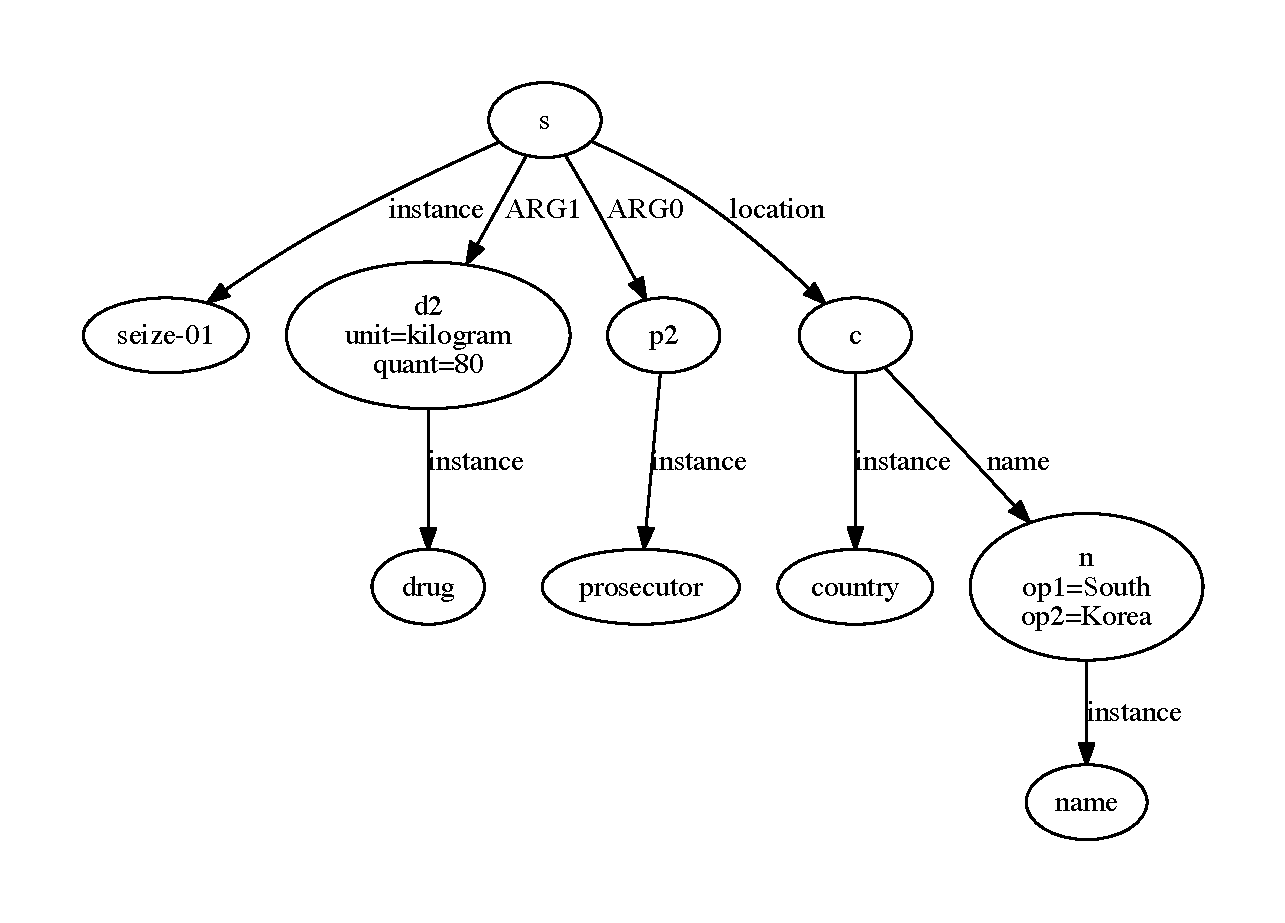
\includegraphics[width=\linewidth]{amr_example.pdf}
\caption{Example AMR in Graphical Form}
\label{fig:amr_example}
\end{figure}

As an example from our dataset, the sentence ``A prosecutor in South Korea seized 80
kilograms of drugs'' would have the following first-order logical form (Figure \ref{fig:amr_example_logical}) and AMR
representation (Figure \ref{fig:amr_example}).

\subsection{Discourse Planning}

In Reiter and Dale's {\em Building Applied Natural Language Generation Systems}, they outline a 6-module pipeline for an NLG system. The second task in this system is Discourse Planning, which they describe as the process of imposing ordering and structure over the set of messages to be conveyed \cite{applied_nlg}. The order of pieces of information in text is not random; rather authors impose a structure on the messages for reasons such as: making the text easier to understand, highlighting the relationships between messages in the text, or stylistic preferences.When making an argument, authors must order the messages so that readers can see the logical implications from one message to the next; if the ordering of the messages were scrambled, readers may fail to understand the argument, even though the same set of information was communicated.

In addition to just logical implication, adjacent sentences can have many different types of relationships with each other, referred to as {\em discourse relations}. A commonly used set of discourse relations are those proposed by {\em Rhetorical Structure Theory} (RST) \cite{rst}. RST defines 32 discourse relations across 3 categories: ``Presentational Relations'', ``Subject Matter Relations'', and ``Multinuclear Relations''.

In applied systems, discourse planning is usually implemented through either schema-based systems or AI planning systems \cite{applied_nlg}. In schema-based systems, messages are given class labels, and are substituted into the appropriate slots which have been predefined in each schema. AI planning is a more general solution in which planning operators are associated with discourse relations, and then off-the-shelf planners can be used to construct a valid discourse plan \cite{hovy1993automated}\cite{paris1990natural}.

\section{Related Work}

Early work by Kukich described a system for ``knowledge-based report generation'' in which manually specified domain rules were used to merge database facts into higher level messages, which were then ordered by a discourse module \cite{kukich1983knowledge}. The ordered output could later be passed to generation system to build a report. Work by Paris in 1990 and Hovy in 1993 introduced the idea of using AI Planners to generate discourse plans. They focused on finding explicit discourse relations between messages and using planners to generate an ordering which was allowed under the constraints of the discourse relations identified \cite{paris1990natural}\cite{hovy1993automated}. 

More recently, Duboue and Mckeown applied Machine Learning (ML) approaches to discourse planning. In \cite{duboue2001empirically}, they present an algorithm to learn ordering constraints among facts. In \cite{duboue2002content}, they build upon this work, using evolutionary algorithms to learn the tree representation of a planner. Although these systems seek to generate valid discourse plans, they do not use a scoring function to choose the `best' among the many valid plans that are available. Dimitromanolaki and Androutsopoulos used ML techniques to learn such a scoring function \cite{learning_to_order_facts}. They train a pipeline of classifiers, where each classifier chooses the next fact to be added to a domain-specific paragraph. In order to train this pipeline, Dimitromanolaki and Androutsopoulos assumed a fixed $k$ number of sentences per paragraph (in their paper $k=6$).

Our work differs from this prior research in four major ways: (1) It is strictly at a semantic level, and the semantic representation is general-purpose. Our entire pipeline is built upon AMR semantics, rather than natural language `facts', meaning the internal entities and their relations can be reasoned about. (2) Higher-level messages are constructed as part of the discourse planning process. While other systems work at the individual fact level, our system seeks to group facts into higher level sentential messages that are ordered by our discourse module. The order of sentential units should be dependent on the information they contain, therefore the merging procedure must occur before or during the discourse planning. (3) Our system does not explicitly model the discourse relations between units. (4) Our system imposes no limit on the number of sentences in a given paragraph.

\section{Data}
\label{sec:data}

The dataset for this research was the AMR ``proxy" dataset - a corpus of
AMR-annotated sentences obtained from newswire data. Since the source text of
the articles was unavailable, we used a sliding window approach to generate
``paragraphs" of size $k$ from the articles. For an article with $n$ sentences,
we could generate paragraphs containing sentences $(s_1,s_2,\ldots,s_k),
(s_2,s_3,\ldots,s_k,s_{k+1}), \ldots (s_{n-k},s_{n-k+1},\ldots,s_n)$.

After applying the sliding window function, our training set had 1676 ``paragraphs" of size $k=5$, and our test set had 214 paragraphs.

\section{Preprocessing}
Before we can feed our dataset through our featurizer and training/test pipeline, we have to apply various transformations to it: the first two are to ensure uniform sentence semantics and the third is to build our paragraph semantics.

\subsection{ARG-of Reversal}
The typical annotation for a sentence is the one shown in Figure \ref{fig:amr_example}. However, due to the annotation format, it is sometimes easier for annotators to add reversed edges. For example, in Figure \ref{fig:amr_example}, instead of adding the edge: (`s', `p2', `ARG0'), an annotator could have added (`p2', `s', `ARG0-of'), resulting in Figure \ref{fig:amr_example_argof}. To fix this, we just reverse any such edge and change the label from `ARGN-of' to `ARGN'.

\begin{figure}
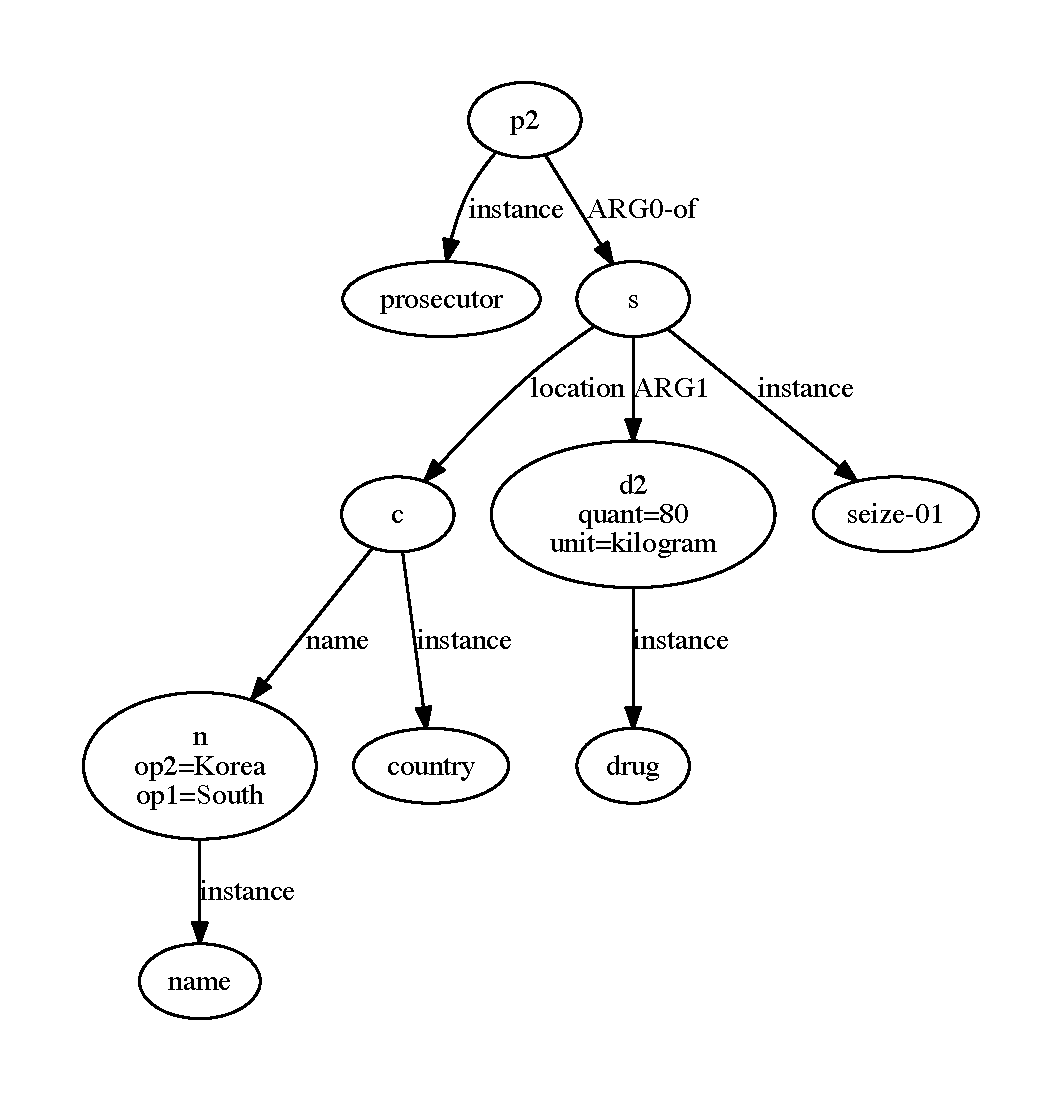
\includegraphics[width=\linewidth]{amr_example_argof.pdf}
\caption{AMR with Reversed Edge}
\label{fig:amr_example_argof}
\end{figure}

\subsection{Translation of `and' Semantics}
The next issue that we had to address in the sentence semantics was the way `and' is handled in AMR. For ease of annotation when `and' occurs in a sentence, an `and' instance is created with everything being `anded' together as its children. Then this `and' instance is used as the argument wherever one of the instances children would have been before. For example, if instead our example sentence were ``A prosecutor in South Korea seized 80 kilograms of drugs and dozens of weapons.'', we would have the AMR graph shown in Figure \ref{fig:amr_example_and} instead of the one in Figure \ref{fig:amr_example}.

\begin{figure}
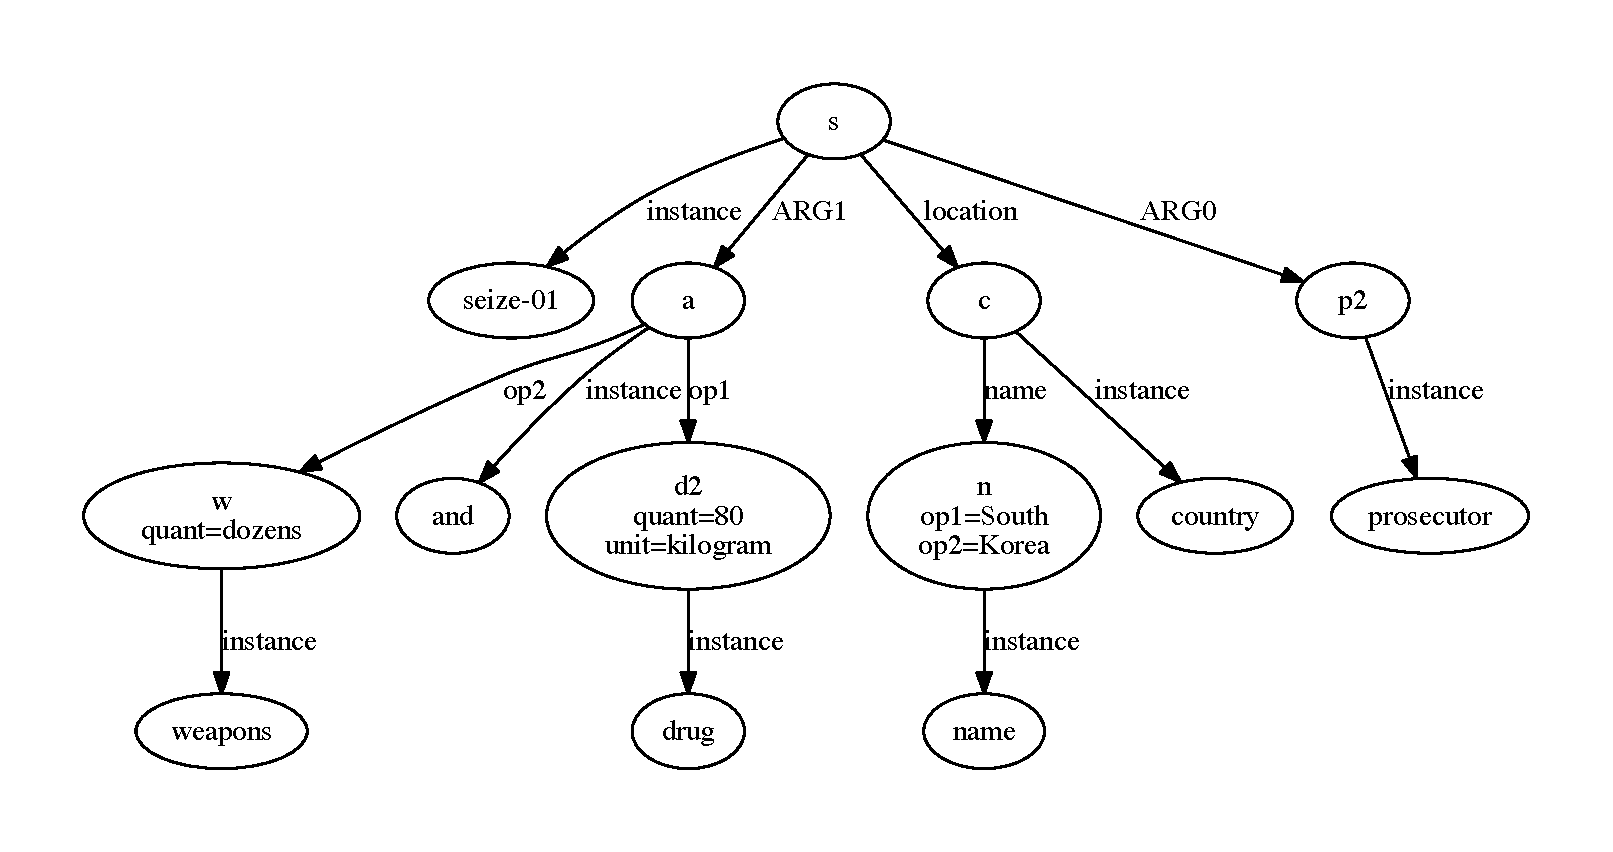
\includegraphics[width=\linewidth]{amr_example_and.pdf}
\caption{AMR with `and' Instance}
\label{fig:amr_example_and}
\end{figure}

While this representation is not necessarily {\em wrong}, the choice to `and' these two entities together was syntactic, not semantic. A strictly semantic representation of this sentence should contain the information: there is a prosecutor, there are drugs, there are weapons, the prosecutor seized the drugs, and the prosecutor seized the weapons. In a generation process, this could be realized as one sentence (``A prosecutor in South Korea seized 80 kilograms of drugs and dozens of weapons.'') or two sentences (``A prosecutor in South Korea seized 80 kilograms of drugs. The prosecutor also seized dozens of weapons.''). Since we ultimately want to look at how information in paragraphs is grouped into sentences and then ordered, we need to translate these `and' semantics back to a strictly semantic representation; otherwise, we have already partially encoded our information grouping.

To recover the actual semantics from the `and' semantics, we must make one copy of the subgraph that the `and' instance is an argument to for each child of the `and' instance. Then, for each copy, we delete the `and' instance and replace it with the child. This algorithm is written formally in algorithm \ref{alg:translate_and_semantics}.

When we apply this algorithm to our semantic graph in figure \ref{fig:amr_example_and}, a new `seize-01' instance is made with the `drugs' instance as ARG1 and another with the `weapons' instance as ARG1. This resulting graph is shown in Figure \ref{fig:amr_example_and_removed}.

\begin{algorithm}
\caption{Translate `and' Semantics}
\label{alg:translate_and_semantics}
\begin{algorithmic}[1]
%require: amr graph
\REQUIRE AMR Graph $G = (V, E)$

% While the graph still has and instances
\WHILE{$|G.and\_instances| > 0$}
    % and_instance = first and instance in topological ordering of G.and_instances
    \STATE $a \gets$ first and\_instance in topological ordering of $G$.and\_instances

    % S = subgraph formed by performing a breadth first search following parent edges from and_instance upwards to roots
    \STATE $S \gets$ subgraph formed by performing a breadth first search following parent edges from $a$ upwards to roots

    % for each child of the and instance
    \FOR{$c \in$ children($a$)}
        % copy S
        \STATE $S' \gets copy(S)$

        % replace and_instance in S with child
        \STATE replace $a$ with $c$ in $S'$

        % add copy to graph
        \STATE $G \gets G \cup S'$
    \ENDFOR
    % delete and_instance and S from graph
    \STATE remove $a$ and $S$ from $G$
\ENDWHILE
% return G
\RETURN $G$
\end{algorithmic}
\end{algorithm}

\begin{figure}
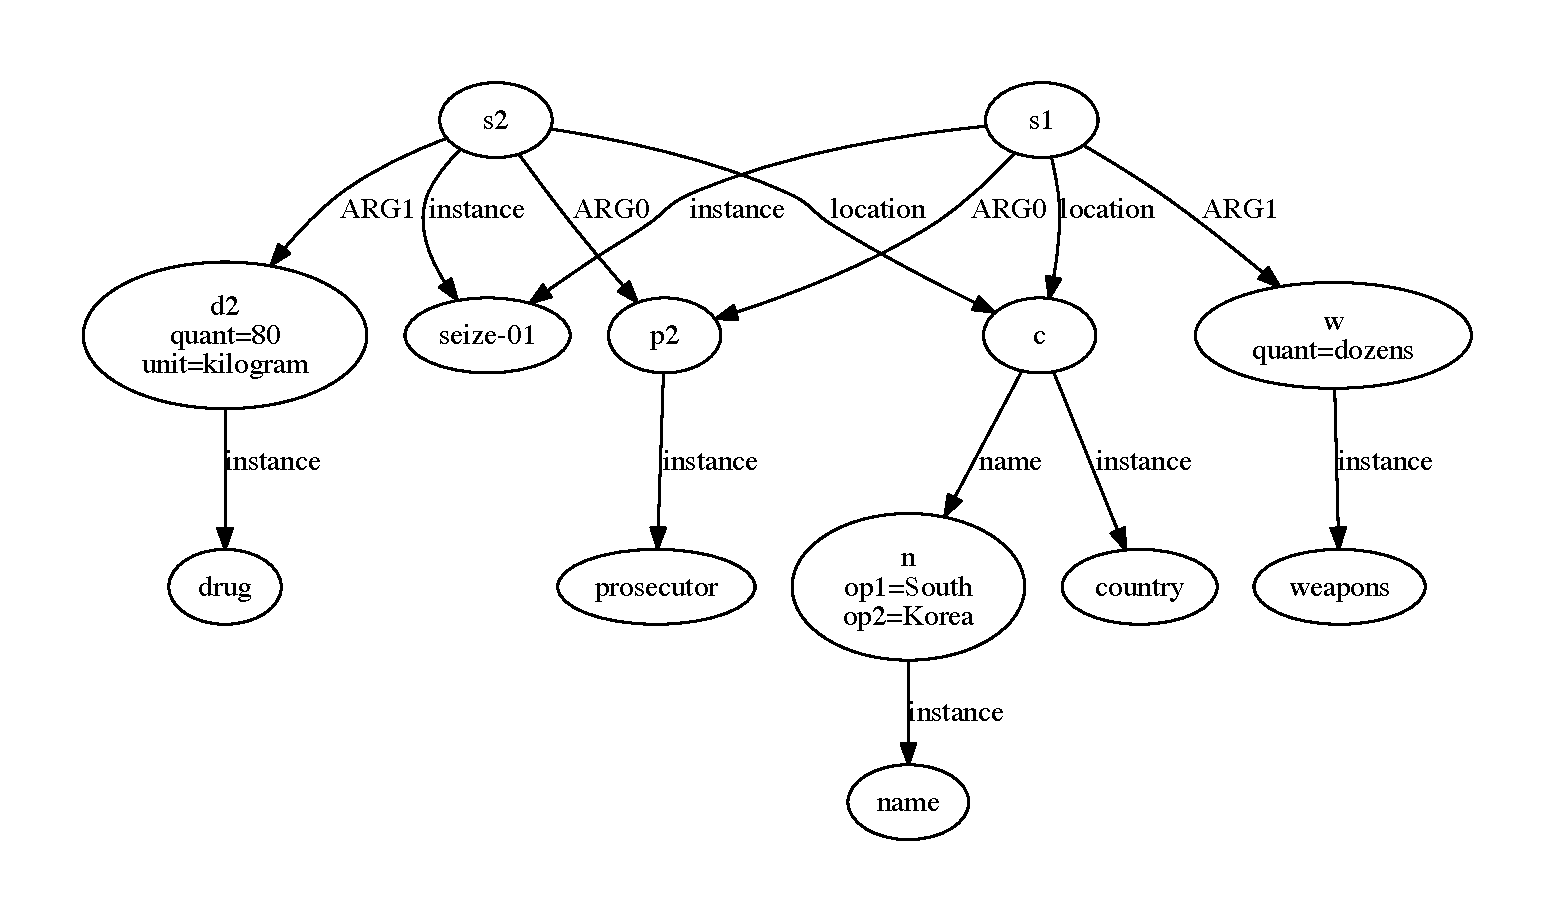
\includegraphics[width=\linewidth]{amr_example_and_removed.pdf}
\caption{AMR with Translated `and' Instance}
\label{fig:amr_example_and_removed}
\end{figure}

\subsection{Graph Merging}
After the semantic graphs have been preprocessed for each sentence, they have to be merged together to form a semantic graph representing all of the information communicated by the paragraph. The only complication is deciding if two entities in separate sentences are the same. For example if we are merging the sentences ``The red dog chased the cat. Afterwards, the dog slept.'', the two dogs should be recognized as the same entity. However, if the sentences were ``The red dog chased the cat. The black dog slept.'', the two dogs should be recognized as separate. 

We define two nodes $u, v$ as {\b equivalent} if they are two `concept' nodes with the same label, or they have no conflicting attributes and no conflicting children. Formally:

\[
    equiv(u,v) = \left\{\begin{array}{lr}
    u.\text{label} = v.\text{label}, & u,v \text{ `concepts'} \\
    \forall k \text{ attribute of } u \text{ and } v, u.\text{attr}[k] = v.\text{attr}[k] \text{ } \land, & \text{else} \\
    \forall e,f \text{ childedge of } u,v \text{ with same label, } equiv(e.\text{child}, f.\text{child}) & \\
    \end{array}\right\}
\]

To merge two sentences, we use our node equivalence function in addition to algorithm \ref{alg:merge_graphs}. Since this algorithm returns a new, merged graph, we can continually apply it to a list of sentences as a reduction function, resulting in a semantic paragraph graph. Figure \ref{fig:amr_example_3_merged} shows the resultant semantic paragraph graph of the following piece of text: ``A prosecutor in South Korea seized 80 kilograms of drugs. The prosecutor disposed of the drugs. South Korean media stated the drugs originated from North Korea.'' We will continue to use this paragraph as an example throughout the paper.

On potential issue arises when a node in one graph has multiple equivalent nodes in the second graph. This can be caused by annotation errors (i.e. a `name' attribute is annotated ``John F. Kennedy'' in one sentence and ``JFK'' in another) or underspecification (i.e. there are two dogs in the world and the next sentence simply refers to ``the dog''). When this happens, there is no clear resolution, so we drop the errant paragraph from our dataset.

\begin{algorithm}
\caption{Merge Two Sentence Semantic Graphs}
\label{alg:merge_graphs}
\begin{algorithmic}[1]
\REQUIRE Two AMR Graphs $G, H$

\FOR{$u \in H.\text{nodes}$}
    \STATE $equiv\_nodes \gets \{v \mid v \in G.\text{nodes} \land equiv(u,v)\}$
    \IF{$|equiv\_nodes| = 0$}
        \STATE $G.\text{nodes} \gets G.\text{nodes} \cup \{\text{safe\_rename}(G, u)\}$
    \ELSIF{$|equiv\_nodes| = 1$}
        \STATE $equiv\_nodes[0].\text{attr} \gets equiv\_nodes[0].\text{attr} \cup u.\text{attr}$
    \ELSE
        \STATE Raise Ambiguity Error
    \ENDIF
\ENDFOR

\STATE $G.\text{edges} \gets G.\text{edges} \cup H.\text{edges}$

\RETURN $G$
\end{algorithmic}
\end{algorithm}

\begin{figure}
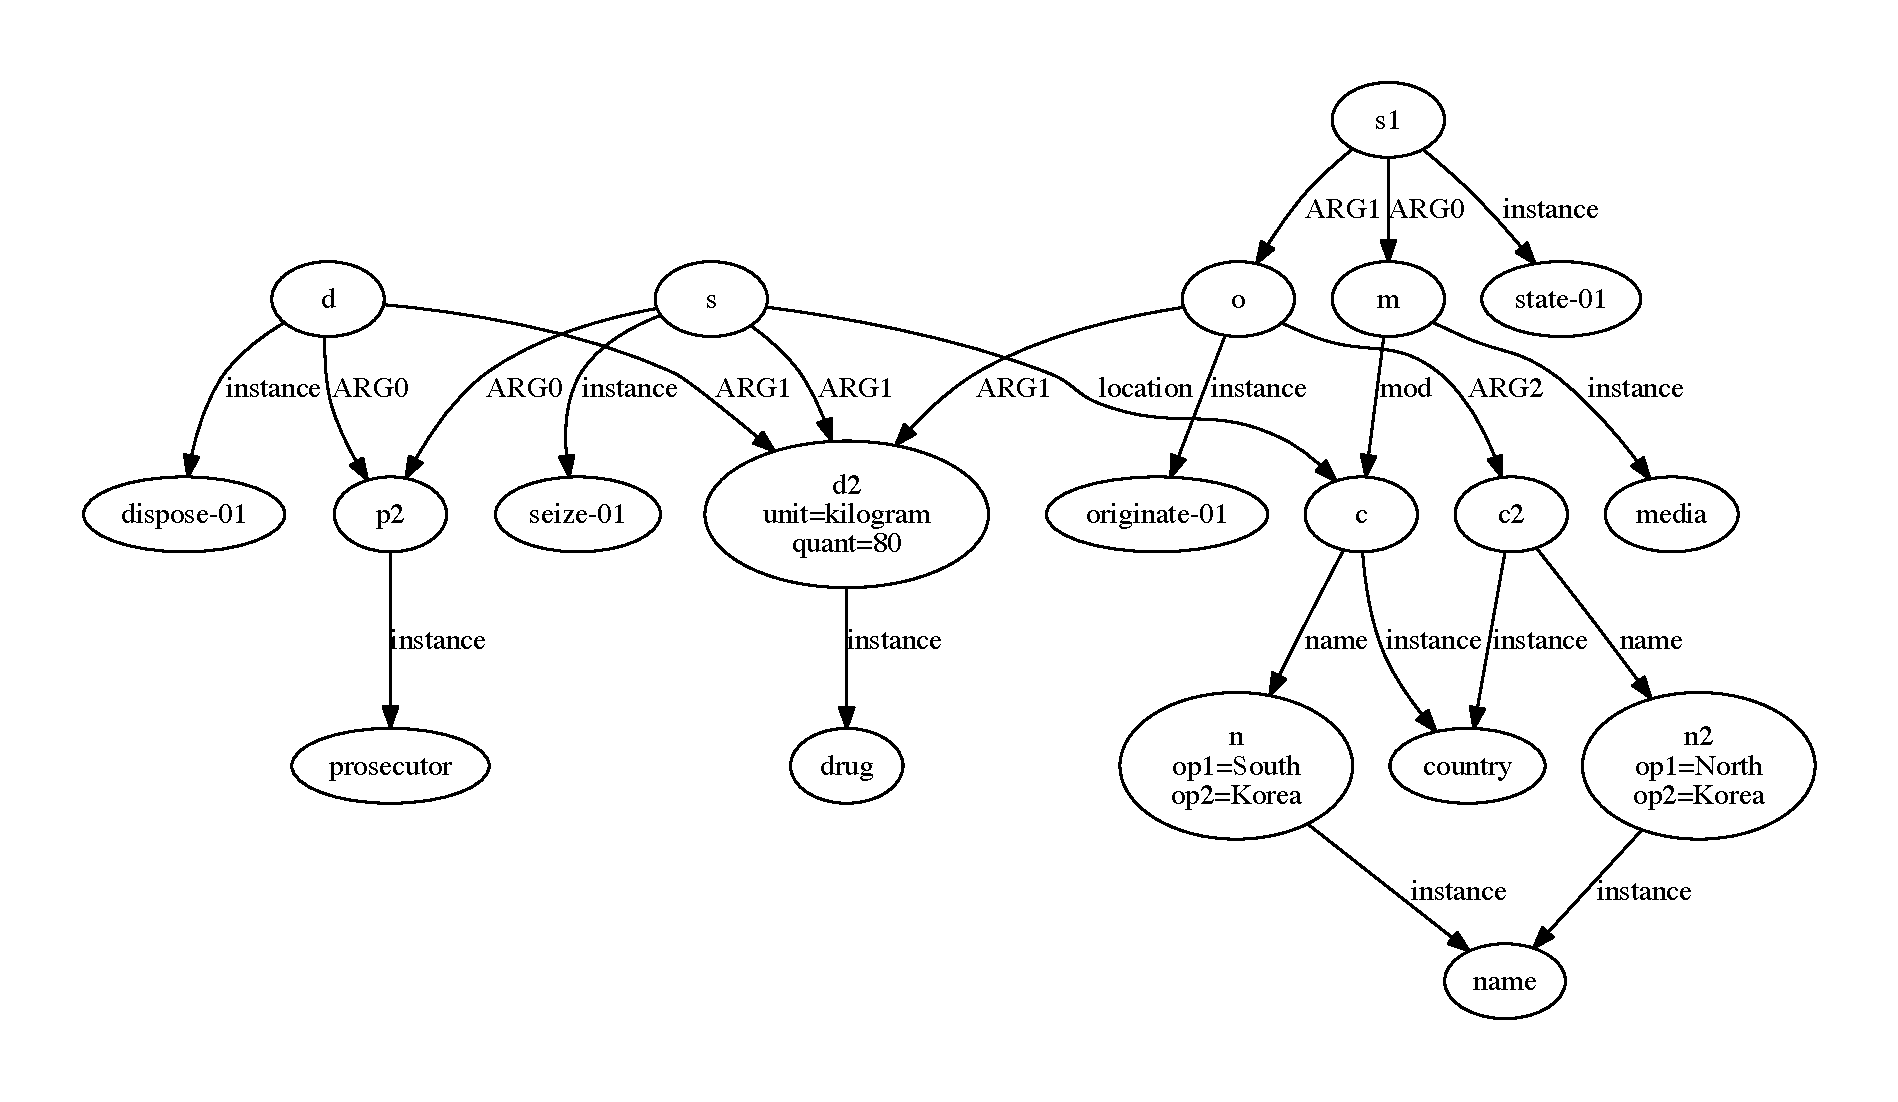
\includegraphics[width=\linewidth]{amr_example_3_merged.pdf}
\caption{Merged AMR Graph of Three Sentences}
\label{fig:amr_example_3_merged}
\end{figure}

\section{System Architecture}

From a high level, our system is a pipeline, which takes as input an AMR representation
of all information that is to be communicated, and outputs a
sequence of AMR representations, which are the AMRs representing a sequence of sentence semantics that could be used to communicate the 
information set.

To accomplish this task, we split the problem into two subproblems: (1)
subgraph selection and (2) subgraph ordering.

For each subproblem, a scoring function was trained to evaluate the ``goodness" of
a given partitioning or ordering, depending on the problem. To find the best
possible partitioning or ordering, we use a greedy search optimization
procedure, which is described more fully in ``Discrete Optimization".

\subsection{Subgraph Selection}
\subsubsection{Problem Description}

Subgraph selection solves the problem of splitting an AMR graph into a set of
subgraphs which are optimal by some criterion, such that the union of the
subgraphs is the original graph. Said more plainly, the problem is to split the paragraph-level semantic graph into groups of information
which are sentence-level semantic graphs.

There are $2^{|E|}$ subgraphs for a paragraph graph with $|E|$ edges. If we consider every set of $N$ subgraphs, we would have to consider $N^{2^{|E|}}$ sets of subgraphs! Obviously this is infeasible. Fortunately, we can exploit the natural language characteristics of a semantic graph to dramatically reduce the number of subgraph sets we have to consider. 

First, we define a {\em fact} in our semantic graph as the subgraph formed by performing a graph-traversal from a root of the graph (that is, a node with no parents). An example is shown in Figure \ref{fig:amr_example_3_merged_s1_highlighted}. By design, the roots of an AMR graph will be verb instances; therefore, we can intuitively think of the rooted graph traversal as a verb + the required graph pieces to fulfill the verb's arguments. Because a syntactically correct sentence requires a verb and its arguments, a {\em fact} is the the smallest piece of a graph that could be used to fully specify the semantics of a sentence. Let $F$ refer to the set of all facts in our graph.

\begin{figure}
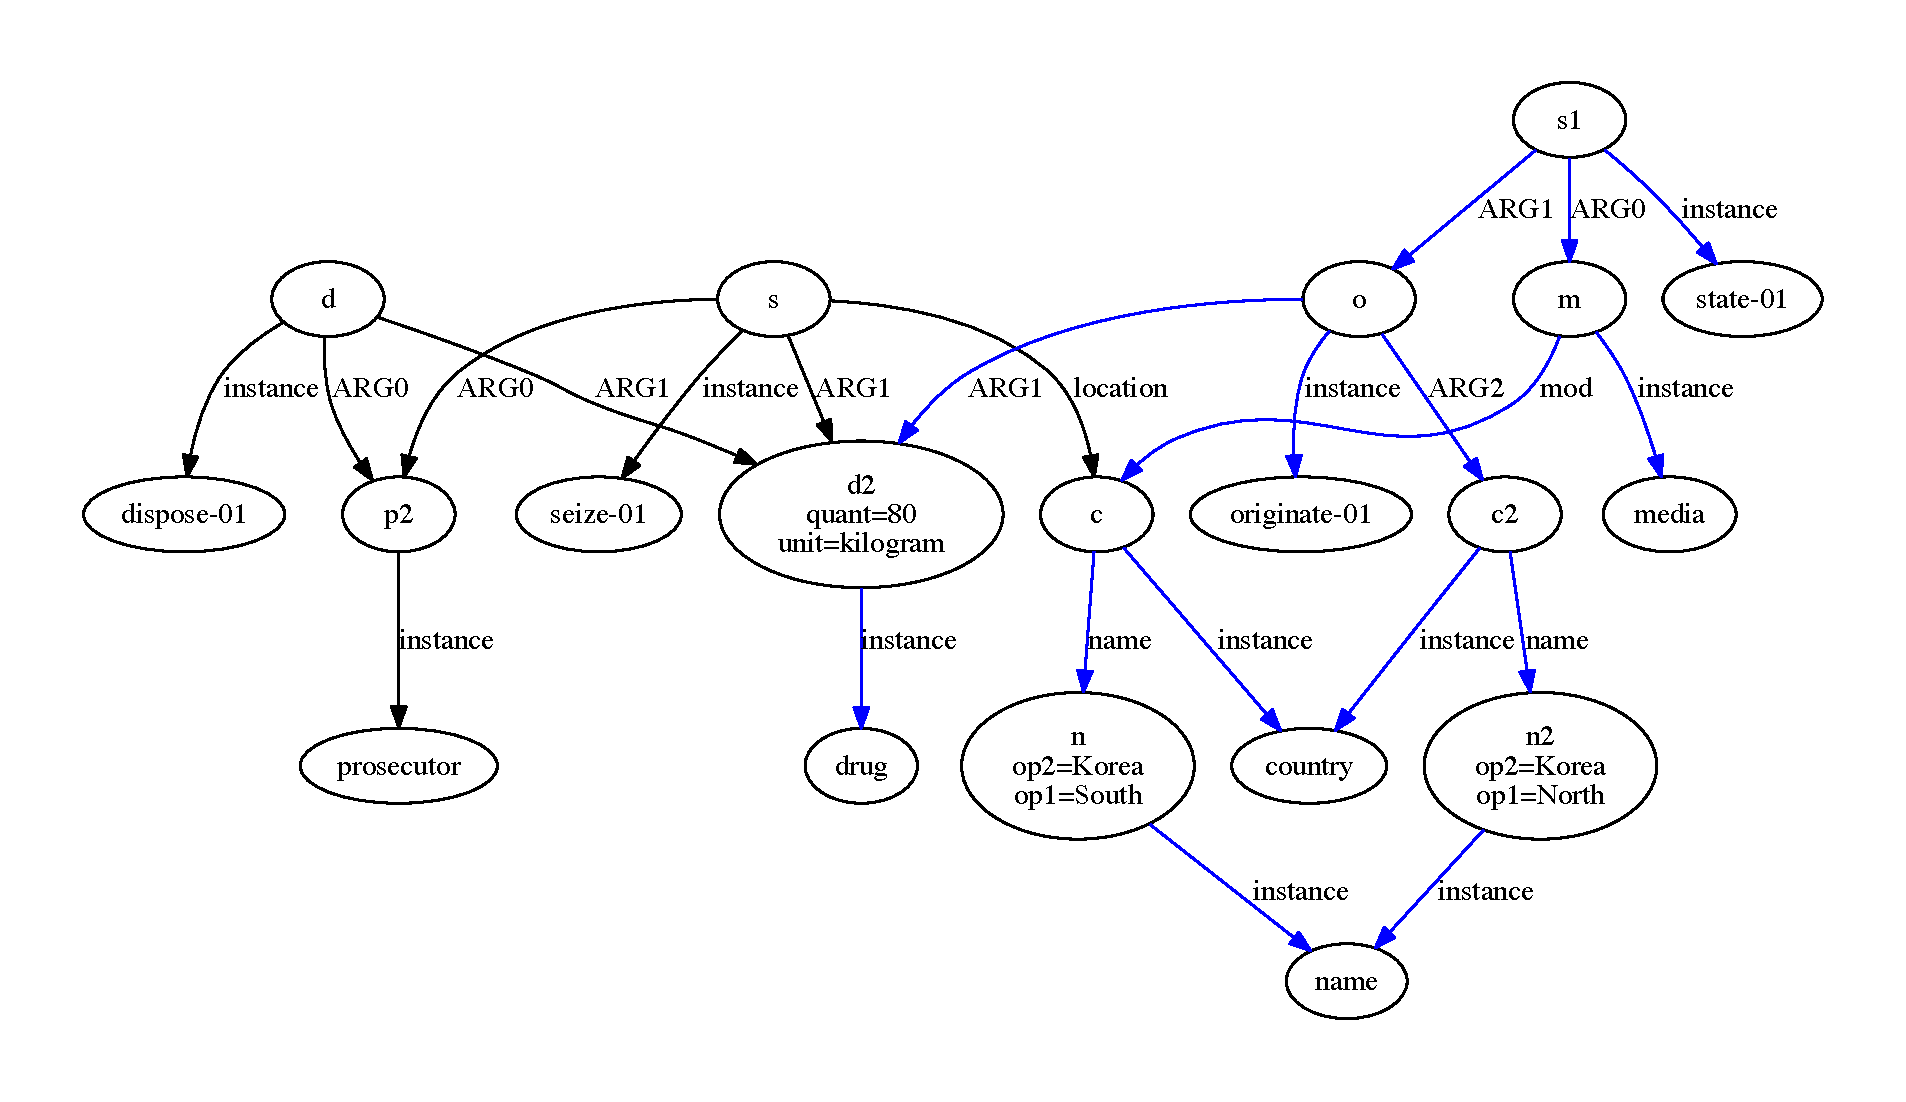
\includegraphics[width=\linewidth]{amr_example_3_merged_s1_highlighted.pdf}
\caption{AMR Graph with fact rooted by `s1' highlighted. Two other facts are present, rooted by `d' and `s'.}
\label{fig:amr_example_3_merged_s1_highlighted}
\end{figure}

Given $F$, our set of facts, and the assumption that we do not want to say the exact same thing twice, we can reduce our search-space to the set of partitions of $F$ from size 1 to $|F|$ (a single group with $|F|$ facts to $|F|$ groups each with 1 fact). The size of our candidate set is now given by $B_{|F|}$, where $B_i$ is the $i^{\text{th}}$ Bell number.

\subsubsection{Training}
Our problem then is to find the best partition from the $B_{|F|}$ candidates. To do this, we trained a scoring function using a logistic regression model with class-weighted instances. We assumed that the fact-partition given by the sentences of a paragraph was correct, and gave it a label of $1$. This means that we had only positive examples in the training set, so we added negative examples by sampling $k$ other valid partitions, giving each a label of $0$.

Table \ref{tab:subgraph_selection_features} lists the features extracted for each candidate partition. To determine subgraph similarity, we used
Jaccard similarity, defined to be:
$$J(A,B) = \frac{\lvert A \cap B \rvert}{\lvert A \cup B \rvert}$$

\begin{table}[H]
\centering
\caption{Features used by subgraph partition scorer}
\label{tab:subgraph_selection_features}
\begin{tabular}{@{}ll@{}}
\toprule
\textbf{Feature}                      & \textbf{Weight} \\ \midrule
\# groups in partition                & 10.30     \\
\# groups in partition squared        & -1.18     \\
mean \# facts per partition           & 1.09      \\
max \# facts per partition            & -0.21     \\
min \# facts per partition            & 0.12      \\
std\_dev \# facts per partition       & 0.20      \\
mean pairwise subgraph similarity     & -18.66    \\
min pairwise subgraph similarity      & 1.77      \\
max pairwise subgraph similarity      & -0.39     \\
std\_dev pairwise subgraph similarity & -7.56     \\
mean pairwise verb set similarity     & -1.03     \\
min pairwise verb set similarity      & 0.04      \\
max pairwise verb set similarity      & 0.90      \\
std\_dev pairwise verb set similarity & -0.17     \\ \bottomrule
\end{tabular}
\end{table}

\subsubsection{Test}

To test the Subgraph Selection scorer, we started with the 214 partitions in our test dataset (each with label 1), and for each one sampled a random partition (with label 0), resulting in a class-balanced test dataset with 428 instances. Features were generated for each instance and the test set was passed through the classifier. The evaluation metrics are reported in table \ref{tab:subgraph_selection_eval}. The classifier performs very well in isolation; this is expected as it is differentiating partitions between ``actual subgraph partition" and ``random subgraph partition''.

In addition to evaluating the test set, we can inspect the feature weights in Table \ref{tab:subgraph_selection_features} to get an idea of what the scoring function is doing. Looking at the first two features, we see that very small and very large paragraphs are penalized (since the ``number of sentences'' feature is positive but the square is negative). After that, we see the two most important features are the mean and standard deviation of the pairwise subgraph similarity. Both features have large negative values. The large negative value on the mean pairwise subgraph similarity implies that the classifier prefers paragraphs for which similar facts are grouped into the same sentence, rather than spread throughout the paragraph. The negative value on the standard deviation implies that the classifier prefers a uniform rate of new information introduced in each sentence.

\begin{table}[H]
\centering
\caption{Evaluation Metrics for Subgraph Selection Classifier}
\label{tab:subgraph_selection_eval}
\begin{tabular}{@{}lllll@{}}
\toprule
\textbf{Precision} & \textbf{Recall} & \textbf{f1-score} & \textbf{auc} & \textbf{support} \\ \midrule
0.93               & 0.93            & 0.93              & 0.98         & 428              \\ \bottomrule
\end{tabular}
\end{table}

\subsection{Subgraph Ordering}
\subsubsection{Problem Description}

Once we have split our semantic graph into a partition of $p$ sentence graphs, there are
$s!$ ways to order the sentences. Ideally, there exists some ordering of the
sentences that communicates the ideas of the merged graph in the best possible
way. Subgraph ordering is the problem of finding this optimal ordering.

\subsubsection{Training}

Once again, we assumed that the ordering of sentences in the dataset was the
optimal ordering for that paragraph, so we needed to create non-optimal
examples to train on as well. This was done by randomly generating
$k=20$ sentence reorderings for each paragraph.

We trained a Ridge regression model on the dataset to predict the Kendall Tau Distance of the ordering
(the distance between a given ordering and the optimal). This is in accordance with prior work, suggesting
the use of this metric \cite{lapata2006automatic}.

As noted in Related Work, our ordering model does not require the number of
sentences to be fixed to a particular value. If it were to impose such a
requirement, then the subgraph selection, which is further upstream in our
pipeline, may not be able to find its optimal partitioning simply because it
was a partitioning into a different number of sentences. As a result, our model
could not rely on any features that deal with particular sentences (e.g. the
similarity between the second and fifth sentences). So, we tried to use
features that would generalize to paragraphs of any length, but would still
vary with the ordering of those sentences within the paragraph. To ensure we 
had the same number of features for each instance, all features had to be summarized (mean, standard deviation, min, max) over the
paragraph. Features included the Jaccard similarity between adjancent
sentences, between sentences that are two sentences apart, and the Jaccard
similarity between the union of adjacent sentences and the overall paragraph.
Table \ref{tab:order_features} summarizes the features used for subgraph ordering.

\begin{table}
\centering
\label{tab:order_features}
\begin{tabular}{|r|c|c|}
\hline
Feature & \\ \hline\hline
Pairwise Jaccard & Jaccard similarity of the AMR graphs for sentences $s_i,s_{i+1}$ \\ \hline
Two-apart Jaccard & Jaccard similarity of the AMR graphs for sentences $s_i,s_{i+2}$ \\ \hline
Pairwise node Jaccard & Jaccard similarity of just the vertex sets for sentences $s_i,s_{i+1}$ \\ \hline
Combined Jaccard & Jaccard similarity between the paragraph AMR and $s_i \cup
s_{i+1}$ \\ \hline
\end{tabular}
\caption{Description of features used by Subgraph Ordering Classifier}
\end{table}

\begin{table}
\centering
\begin{tabular}{|r|c|c|}
\hline
Feature & Weight \\ \hline\hline
mean pairwise Jaccard & -5.00 \\ \hline
std\_dev pairwise Jaccard & -0.33 \\ \hline
min pairwise Jaccard & 2.61 \\ \hline
max pairwise Jaccard & 1.56 \\ \hline
mean two-apart Jaccard & 4.19 \\ \hline
std\_dev two-apart Jaccard & 7.77 \\ \hline
min two-apart Jaccard & 2.94 \\ \hline
max two-apart Jaccard & -4.35 \\ \hline
mean pairwise node Jaccard & -0.94 \\ \hline
std\_dev pairwise node Jaccard & 4.50 \\ \hline
min pairwise node Jaccard & 1.14 \\ \hline
max pairwise node Jaccard & -1.95 \\ \hline
mean combined Jaccard & 0.48 \\ \hline
std\_dev combined Jaccard & -1.85 \\ \hline
min combined Jaccard & -0.58 \\ \hline
max combined Jaccard & 0.82 \\ \hline
\end{tabular}
\caption{Features used by Subgraph Ordering Classifier}
\end{table}

Inspecting these feature weights, we see that the most important feature is the
standard deviation for the two-apart Jaccard similarity. Having such a large
positive value indicates that the scorer prefers paragraphs that do not have
uniform overlap between a sentence and the sentence which comes second after
it. Next is the mean pairwise Jaccard similarity, which gets penalized heavily.
This would indicate that the scorer prefers paragraphs that don't have much
overlap between adjacent sentences. At first, this does not seem to make much
sense at all, as one would expect to want to have some information overlap
moving from sentence to sentence through a paragraph. However, we also observe
that the standard deviation for pairwise similarity is penalized. So, the
scorer also prefers orderings which make the information overlap through the
paragraph more uniform.

\subsubsection{Testing}

For subgraph ordering, we use Kendall's tau metric as our evaluation function.
For each test example, we compute the Kendall tau distance between a random
ordering and the correct ordering, to use as a baseline. Then, we perform a
greedy search discrete optimization as described above using the subgraph
ordering model to compute the scores of the various orderings.

The mean, standard deviation, min, and max for both the baseline and greedy
Kendall tau are reported in Table \ref{tab:order_eval}.

\begin{table}
\centering
\begin{tabular}{|r|c|c|c|c|c|}
\hline
Approach & Mean  & Std.  & Min & Max \\ \hline\hline
Baseline & 5.01 & 2.09 & 0   & 10  \\ \hline
Greedy   & 1.36 & 0.91 & 0   & 5   \\ \hline
\end{tabular}
\label{tab:order_eval}
\caption{Evaluation Metrics for Subgraph Ordering}
\end{table}


\subsection{Discrete Optimization}

In both subproblems, we trained classifiers which assign a score to how ``good"
an instance is with regard to that problem. So, to find the best instance, we
could just enumerate all possible permutations or combinations of the input,
and select the instance which maximizes (or, in the case of subgraph ordering,
minimizes) the classifier's score. However, in both cases, there is an exponential number of possible orderings.
It is not computationally feasible to evaluate each, so we
perform discrete optimization to approach an optimal solution, rather than
enumerating all possible inputs. It is worth noting that in practice, this is
more of a problem for the subgraph selection module, since the number of partitions
returned by the subgraph selector is generally not too large.

For discrete optimization, we implemented a greedy search outlined in Algorithm \ref{greedy_search_alg}.

\begin{algorithm}
\caption{Greedy search procedure}
\label{greedy_search_alg}
\begin{algorithmic}
\STATE Input: $s$ // start state \\
\STATE Input: $classifier$ \\
\STATE $Q \gets [s]$ // queue of states to visit \\
\STATE $opt, optv, oldoptv \gets null, 0, 1$
\WHILE{$Q\neq\emptyset$ and $optv \neq oldoptv$}
    \STATE $S \gets \{s: s \in Q \}$
    \STATE $Q \gets \emptyset$
    \STATE $oldoptv \gets optv$
    \FORALL{$s \in S$}
        \STATE $N \gets neighbors(s)$\\
        \STATE Add all elements of $N$ to $Q$\\
        \IF{$classifier.score(s) > optv$}
            \STATE $opt, optv \gets s, classifier.score(s)$\\
        \ENDIF
    \ENDFOR
\ENDWHILE
\end{algorithmic}
\end{algorithm}

In addition to the greedy search, we experimented with simulated annealing for the
subgraph ordering problem.

\subsection{Pipeline}

To construct the entire pipeline, we trained the subgraph selector and subgraph
orderer separately and combined them via Algorithm \ref{pipeline_procedure}.

\begin{algorithm}
\caption{Full Pipeline}
\label{pipeline_procedure}
\begin{algorithmic}
\STATE Input: $P \gets$ Full AMR representation of paragraph
\STATE Input: $selector \gets$ subgraph selector
\STATE Input: $orderer \gets$ subgraph orderer
\STATE Starting with an initial partition $p$ of $P$, perform discrete
optimization using $selector$ to find an optimal partition $p'$.
\STATE Use $orderer$ to perform a discrete optimization over potential
orderings of the subgraphs in $p'$ to find an optimal ordering $o'$.
\STATE Output the subgraphs $p'$ ordered by $o'$
\end{algorithmic}
\end{algorithm}

To evaluate the pipeline as a whole, we used a revised Kendall's tau metric. 
To score both the selection and ordering simultaneously, we count the number of facts which are out of order.
This accounts for mistakes both in the subgraph selection, where a fact is
placed in the wrong sentence, and in the subgraph ordering, where a sentence
is placed in the wrong order.

\section{Experiments}

We trained the subgraph selector and orderer on our training dataset and
constructed a pipeline as described in Algorithm \ref{pipeline_procedure}.
To establish a baseline, we ran the
pipeline against our test set, but rather than perform discrete optimization,
each optimizer used a random sampling from the possible partitions and 
orderings respectively.

Next, we ran the pipeline again, this time using our discrete optimizations.
We implemented only greedy search for the subgraph selection problem, but ran experiments with
both greedy search and simulated annealing for the subgraph ordering problem.

Table \ref{tab:experiments} summarizes the mean, standard deviation, min and max of the
revised Kendall tau metric for each experiment.

\begin{table}[H]
\centering
\caption{Revised Kendall Tau Metrics}
\label{tab:experiments}
\begin{tabular}{@{}lllll@{}}
\toprule
\textbf{(Selection, Ordering)} & \textbf{Mean} & \textbf{Std. Dev.} & \textbf{Min} & \textbf{Max} \\ \midrule
Baseline, Baseline & 40.97 & 62.38 & 0 & 634 \\
Greedy, Greedy & 36.43 & 61.22 & 2 & 563 \\
Greedy, Annealing & 34.48 & 50.60 & 2 & 411 \\ \bottomrule
\end{tabular}
\end{table}

Looking at these results, we see that performing the discrete optimizations do
yield results that are better than our baseline, and that both greedy search
and annealing give about the same improvement over the baseline for the
subgraph ordering subproblem.

Looking at table \ref{tab:metrics}, we also see that the optimized pipeline
prefers fewer sentences per paragraph, with marginally more information per
sentence, than the baseline.

\begin{table}[H]
\centering
\caption{Sentence Metrics for the full pipeline}
\label{tab:metrics}
\begin{tabular}{@{}lll@{}}
\toprule
\textbf{(Selection, Ordering)} & \textbf{Mean \# Sentences} & \textbf{Mean \# Facts per Sentence} \\ \midrule
Baseline, Baseline & 6.11 & 2.33 \\
Greedy, Greedy & 5.81 & 2.45\\
Greedy, Annealing & 5.81 & 2.45 \\ \bottomrule
\end{tabular}
\end{table}

\section{Conclusion and Future Work}
This paper has presented a Machine Learning approach to general-purpose discourse planning at a semantic level. We have provided a pipeline that, given a complex semantic representation of information to communicated, selects how to split that information into sentential units, and then selects how to order those sentential units. Both discrete optimization strategies applied to the learned scoring functions resulted in a better information ordering than a random baseline, according to a modified Kendall-Tau distance. The discourse planner presented can be used on any AMR-annotated sentences, rather than domain-specific facts. 

The system currently has two major drawbacks, which represent opportunities for future work:

(1) The evaluation of system such as this ultimately needs to have human involvement, with subjective scoring done by native English speakers. The learned scorers seek to find information groupings and orderings that match those of the input texts; however there is no reason to believe that other groupings/orderings are incorrect. The difficulty in this process is that understanding the semantics of an AMR paragraph a non-trivial task for a human-scorer. These graphs could have hundreds of nodes and edges, representing complex higher-order logic. Without an NLG system built upon AMR semantics it will be incredibly time-consuming for a human annotator. We may be able to build a tool that translates AMR to a more easily understandable language, without having to generate all the way to natural language, allowing more rapid human scoring. 

(2) In our system, information grouping and ordering are treated as separate systems in a pipeline; however, these two tasks should really happen simultaneously. The ordering of information is clearly dependent on how the information is grouped, and the information grouped in a sentence should be dependent on what has already been said (the ordering of sentences beforehand). Since these two tasks are interdependent, we expect a simultaneous system would outperform our pipeline architecture.

\pagebreak
\bibliographystyle{ieeetr}
\bibliography{paper}
\end{document}
